\documentclass{standalone}
\usepackage{tikz}
\usepackage{../mss}
\usepackage{sansmath}

\usetikzlibrary{shapes.geometric,positioning,calc,petri,graphs,fit,backgrounds}
\tikzset{
        node distance=1.35cm and 1.35cm,
        >=latex,
        font=\sf\bfseries\sansmath,
        every edge/.append style={line width=1.1pt}
        textfeld/.style={align=center,minimum height=0.5cm,minimum width=1.5cm},
        pfeil/.style={->,line width=1.1pt},
        box/.style={rectangle,draw,line width=1.1pt,minimum height=1.5cm,minimum width=2.8cm,align=center},
        place/.style={circle,line width=1.1pt,draw=black,minimum size=6mm},
        transition/.style={rectangle,line width=1.1pt,draw=black,minimum size=6mm},
        initial/.style={draw=none},
        module/.style={rectangle,fill=gray!5,line width=1.1pt,inner sep=10pt},
        module label/.style={text=gray!50},
        synchronization/.style={draw,dashed,rounded corners,inner sep=6pt},
        segment/.style={rectangle,draw,dashed,rounded corners=3mm,minimum height=1.5cm,minimum width=2.8cm}
        }
\tikzgraphsset{
    every graph/.style = {use existing nodes}
}
\begin{document}
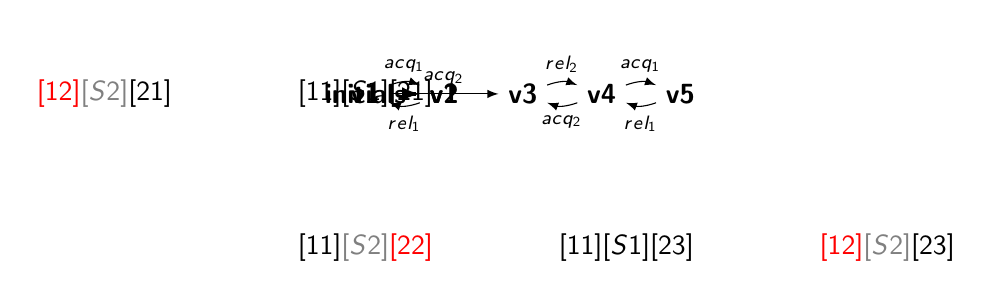
\begin{tikzpicture}
    % before first access of P2 
    \node[] (v1) {$ \segment[11]\segment[S1]\segment[21] $};
    \node[left=of v1] (v2) {\textcolor{red}{$ \segment[12] $}\textcolor{gray}{$ \segment[S2] $}$ \segment[21]$}; % P1 in critical
    \node[below=of v1] (v3) {$ \segment[11]$\textcolor{gray}{$ \segment[S2] $}\textcolor{red}{$ \segment[22] $}}; % P2 in critical
    % after
    \node[right=of v3] (v4) {$ \segment[11] \segment[S1] \segment[23]$}; % Noone in critial
    \node[right=of v4] (v5) {\textcolor{red}{$ \segment[12] $}\textcolor{gray}{$ \segment[S2] $}$\segment[23]$}; % P1 in critical

    \node[initial, above left=3mm and 1.5mm of v1] (initials) {};
    % 
    % 
    \graph{
    v1 ->[bend left=20,edge label={$ \synchronization_{acq_1} $}] v2 ->[bend left=20,edge label={$ \synchronization_{rel_1} $}] v1 ->[edge label={$ \synchronization_{acq_2} $}] v3 ->[bend left=20,edge label={$ \synchronization_{rel_2} $}] v4
    -> [bend left=20,edge label={$ \synchronization_{acq_1} $}] v5 ->[bend left=20,edge label={$ \synchronization_{rel_1} $}] v4 ->[bend left=20,edge label={$ \synchronization_{acq_2} $}] v3
    % start2 ->[edge label={$ proc_2 $}] idle2 ->[edge label={$ req_2 $}] wait2 ->[edge label={$ acq_2 $}] crit2 ->[edge label={$ rel_2 $}, bend left=170] start2
    };

    \graph{
    initials ->[line width=1.2pt] v1
    };


\end{tikzpicture}
\end{document}